\chapter{Symmetric Matrices}

\begin{definition}
    A \textbf{Symmetric} matrix is a matrix A such that $A^{T} = A$.
\end{definition}


\section{Diagonalization of symmetric matrix}

Recall that \textbf{linear independent} does not mean \textbf{orthogonal}. If we say 2 vectors are linear independent, which simply means no scalar c except for 0 can make $v_1 = c v_2$, while orthogonal means the dot product of 2 vectors is zero: $v_1 \perp v_2 \Rightarrow v_1 \cdot v_2 = 0$.

Look carefully at following example:
\begin{eg}
    diagonalize the matrix $A = \begin{bmatrix}
        6 & -2 & -1 \\
        -2 & 6 & -1 \\
        -1 & -1 & 5 \\
    \end{bmatrix}$

    The result is $A = PDP^{-1}$, where $P = \begin{bmatrix}
        -1/\sqrt{2} & -1/\sqrt{6} & 1/\sqrt{3} \\
        1/\sqrt{2} & -1/\sqrt{6} & 1/\sqrt{3} \\
        0 & 2/\sqrt{6} & 1/\sqrt{3} \\
    \end{bmatrix}$, $D = \begin{bmatrix}
        8 & 0 & 0 \\
        0 & 6 & 0 \\
        0 & 0 & 3 \\
    \end{bmatrix}$.
\end{eg}

In the above example, because P is square and has orthogonal columns, according to what we have proved in orthogonal section, P is an \textit{orthogonal} matrix, and $P^{-1} = P ^T$.


\begin{remark}
    Does a symmetric matrix necessarily diagonalizable?
\end{remark}

The answer is yes, will prove this in following theorems. Also, intuitively, a symmetric matrix is similar with a diagonal matrix.

\begin{remark}
    Does a symmetric matrix necessarily has eigenvalues?
\end{remark}

The answer is yes, and we can depend this on the previous question: because it is diagonalizable, then it must have eigenvalues and eigenvectors.

\begin{theorem}\label{theorem: 7.1.1}
    If A is symmetric, then any 2 eigenvectors from different \\ eigenspaces are orthogonal.
\end{theorem}

\begin{proof}
    Suppose matrix A has $\lambda_1, \lambda_2$ as eigenvalues and $v_1, v_2$ as eigenvectors.

    \begin{align*}
        \lambda_1v_1 \cdot v_2 & = (\lambda_1 v_1)^{T} v_2 \qquad(obviously)\\
        & = (Av_1)^T v_2 \qquad(definition of eigen)  \\
        & = v_1^T A^T v_2 \qquad(transpose) \\
        & = v_1^T A v_2 \qquad(definition of symmetric) \\
        & = v_1^T \lambda_2 v_2 \qquad(eigen) \\
        & = \lambda_2 v_1 \cdot v_2
    \end{align*}

    $$\lambda_1 \neq \lambda_2 \Rightarrow v_1 \cdot v_2 = 0$$
\end{proof}

\begin{theorem}\label{theorem: 7.1.2}
    An $n \times n$ matrix A is orthogonally diagonalizable if and only if A is a symmetric matrix.
\end{theorem}

\begin{proof}[Part of proof]
One part of this theorem is easy to prove: if it's orthogonally diagonalizable then it is a symmetric matrix:

(1) What is \textbf{orthogonally diagonalizable}?

An $n \times n$ matrix A is said to be \text{orthogonal diagonalizable} if there are an orthogonal matrix P (a real square matrix whose columns and rows are orthonormal vectors) (with $P^{-1} = P^T$) and a diagonal matrix D such that:
$$A = PDP^T = PDP^{-1}$$

(2) How can we prove such A is symmetric?

Always remember by definition we're going to prove $A^T = A$. Let's apply transpose to A:

$$A^T = (PDP^T)^T = P^{TT}DP^T = PDP^T = A$$
\end{proof}

Another part of the theorem: if symmetric then orthogonally diagonalizable is hard to proof, the book omitted it here.

% ............the end of section............

\section{The Spectral Theorem}

The set of eigenvalues of matrix A is sometimes called the \textit{spectrum} of A.

\begin{theorem}[The Spectral Theorem for Symmetric Matrices]
An \(n \times n\) symmetric matrix A has the following properties:

a. A has n real eigenvalues, counting the multiplicities

b. The dimension of the eigenspace for each eigenvalues \(\lambda \) equals the multiplicities of \(\lambda \) as a root of the characteristic equation

c. The eigenspaces are mutually orthogonal, in the sense that eigenvectors corresponding to different eigenvalues are orthogonal

d. A is orthogonal diagonalizable
\end{theorem}

\begin{proof}
    a. To find eigenvalues for A, we have \(Ax = \lambda x\), to find x, we have \(det(A - \lambda I)= 0\). Because it is an n degree polynomial equation, according to the foundational theorem of algebra, it has n roots.
    
    According to \hyperref[ex: 5.5.24]{this exercise}, \(\lambda\) will be real number, thus we can say it has n real eigenvalues. 

    c. The same with \hyperref[theorem: 7.1.1]{this theorem}.

    d. See \hyperref[ex: 7.1.31]{this exercise}

    b. Follows d.
\end{proof}

\begin{remark}
    What is eigenspace?

    Eigenspace is all solutions of \((A - \lambda I) \vec{x}  = 0\) 
\end{remark}


\begin{remark}
    What is the dimension of eigenspace?

    How many vectors we need to span the eigenspace.
\end{remark}

\begin{problem}[chapter 7.1 exercise 31]\label{ex: 7.1.31}
    Let \(A = PDP^{-1}\), where P is orthogonal and D is diagonal, and let \(\lambda\) be an eigenvalue of A of multiplicity k. Then \(\lambda\) appears k times on the diagonal of D. Explain why the dimension of the eigenspace for \(\lambda\) is k.   
\end{problem}
\begin{proof}
    According to \hyperref[theorem: diagonal theorem]{diagonal theorem}, because A is diagonalizable, implies that P are linear independent eigenvectors of A corresponding to eigenvalues.

    So, P has k eigenvectors corresponding to \(\lambda\). 
\end{proof}


% Quadratic forms, corresponding to chapter 7.2 of the book
\section{Quadratic Forms}

In general, \textbf{quadratic form} is a polynomial with terms all of degree two (\textbf{form}  is another name for a homogeneous polynomial). A homogeneous polynomial is a polynomial whose nonzero terms all have the same degree.

Here is the definition on linear algebra:
\begin{definition}[quadratic form]
    A \textbf{quadratic form} on \(\R^n\) is a function Q defined in \(\R^n\) whose value at a vector x in \(\R^n\) can be computed by an expression of the form \(Q(x) = x^T A x\), where A is an \(n \times n\)  symmetric matrix.      
    The matrix A is called the \textbf{matrix of the quadratic form}. 
\end{definition}

\begin{eg}
    The simplest example of a nonzero quadratic form is \(Q(x) = x^T I x = {\lVert x \lVert}^2\). 
\end{eg}

\subsection{Change of Variable in a Quadratic Form}
\begin{definition}[change of variable]
    If x represents a variable vector in \(R^n\), then a \textbf{change of variable} is an equation of the form

    \(x = Py\) or equivalently, \(y = P^{-1}x\)  \\
    where P is an invertible matrix and y is a new variable vector in \(R^n\). Here y is the coordinate vector of x relative to the basis of \(R^n\) determined by the columns of P. 
\end{definition}
\begin{remark}
    If the change of variable is made in a quadratic form \(x^T Ax\), then
    \[
        x^TAx = (Py)^T A (Py) = y^T P^T APy = y^T(P^TAP)y  \tag{1}
    \]
    and the new matrix of the quadratic form is \(P^T AP\). 
    Since A is symmetric, and \hyperref[theorem: 7.1.2]{this theorem} shows that A can be decomposed of \(P DP^T\), thus we have a diagonal matrix \(D = P^T AP\). 

    The quadratic form (1) becomes \(y^TDy\). 
\end{remark}

\begin{eg}
    Do the change of variable on \(A = \begin{bmatrix}
        1 &  -4 \\
        -4 &  5 \\
    \end{bmatrix}\) 

    1. First let's see the quadratic form. \(\vec{x} = \begin{bmatrix}
        x_1 &  x_2 \\
    \end{bmatrix}\): 
    \[
        x^TAx = x_1^2 - 8x_1x_2 - 5x_2^2
    \]

    2. Try to find P, so we can do the change of variable.

    The eigenvalues and corresponding eigenvectors are:
    \[
        \lambda = 3: \begin{bmatrix}
             2/\sqrt{5} \\
             1/\sqrt{5} \\
        \end{bmatrix};
        \quad
        \lambda = -7: \begin{bmatrix}
             1/\sqrt{5} \\
             2/\sqrt{5} \\
        \end{bmatrix}
    \]

    \begin{remark}
    Notice that we need to normalize the eigenvector, so we have \(P^T = P^\{ -1 \} \).
    \end{remark}

    So we have \(P = \begin{bmatrix}
        2/\sqrt{5} &  1/\sqrt{5} \\
        -1/\sqrt{5} &  2/\sqrt{5} \\
    \end{bmatrix}\)
    and  \(D = \begin{bmatrix}
        3 &  0 \\
        0 &  -7 \\
    \end{bmatrix}\) 

    3. Replace \(x = Py\) and calculate \(x^TAx = (Py)^TA(Py) = y^TP^TAPy = y^TDy = 3y_1^2 - 7 y_2^2\)   

    That's the end of the change of variable.
\end{eg}

\begin{note}
    Quadratic form is very natural in real day problems. 

    We should know that \(Q(x) = x^TAx\)  is simply \(Q(x) = \sum_{i=1}^n \sum_{j=1}^n a_{ij}x_ix_j\). 

    And change of variable makes the calculation easier.

    I would think that this subsection is a small application for symmetric matrices.

    Also notice the change of variable has no cross-product term.
\end{note}

The above example has shown that:
\begin{theorem}[The Principle Axes Theorem]\label{theorem: Principle Axes Theorem}
    Let A be an \(n \times n\) symmetric matrix. Then there is an orthogonal change of variable, \(x = Py\), that transforms the quadratic form \(x^TAx\) into a quadratic form \(y^TDy\) with no cross-product term.    
\end{theorem}

\subsection{A Geometric View of Principle Axes}
For a general form of \(Q(x) = x^TAx\), suppose \(A = \begin{bmatrix}
    a_{11} &  a_{12} \\
    a_{21} &  a_{22} \\
\end{bmatrix}\), we have \(Q(x) = a_{11} x_1^2 + (a_{12}+1_{21})x_1x_2 + a_{22}x_2^2\).  

Let \(c\) be a constant and let's show all x in \(\R^2\) satisfy \(Q(x) = c\):  

If \(A\) is a diagonal matrix, then we can always get the form of an ellipse (\(\dfrac{x_1^2}{a^2} + \dfrac{x_2^2}{b^2} = 1, a > b > 0\)) or a hyperbola (\(\dfrac{x_1^2}{a^2} - \dfrac{x_2^2}{b^2} = 1, a > b > 0\)):
\begin{figure}[h]
    \centering
    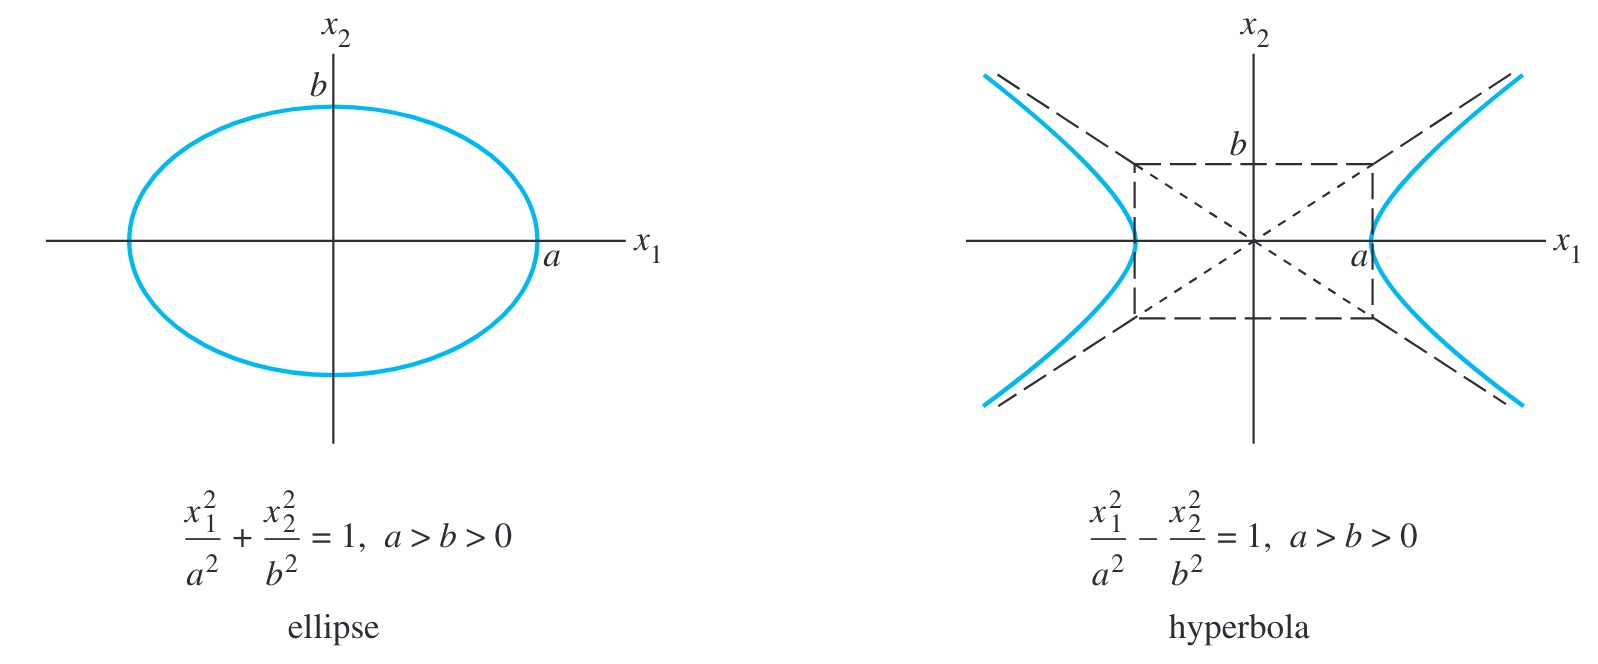
\includegraphics[width=\textwidth]{standard-ellipse-hyperbola}
    \caption{An ellipse and a hyperbola in standard position}
    \label{fig:standard-ellipse-hyperbola}
\end{figure}

If \(A\)  is not a diagonal matrix, then the graphs will be rotated out of the standard position:
\begin{figure}[h]
    \centering
    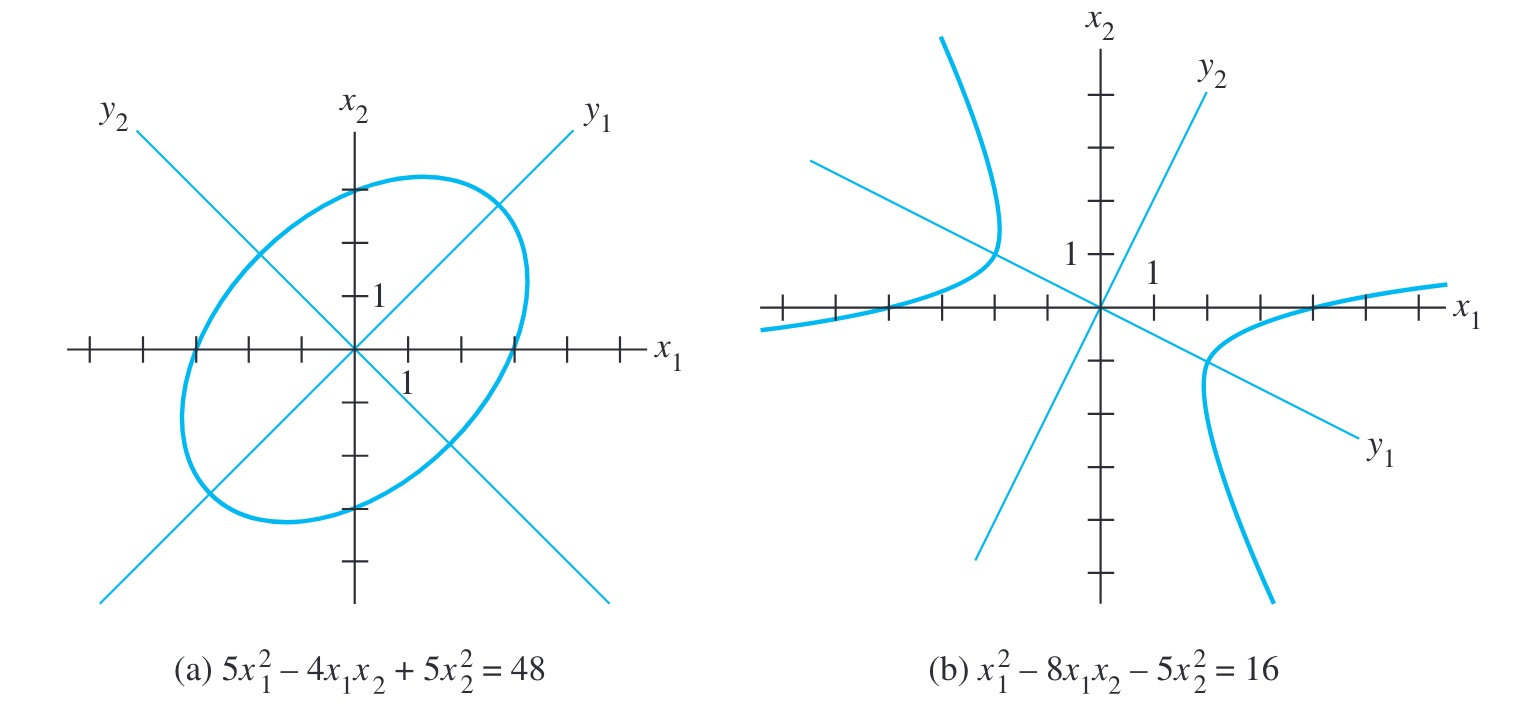
\includegraphics[width=\textwidth]{non-standard-ellipse-and-hyperbola}
    \caption{An ellipse and a hyperbola not in standard position}
    \label{fig:non-standard-ellipse-and-hyperbola}
\end{figure}

\subsection{Classifying Quadratic Forms}
When A is an \(n \times n\) matrix, the quadratic form \(Q(x) = x^T Ax\) is a real-valued function with domain \(R^n\).   

\begin{definition}
    A quadratic form Q is:
    \begin{itemize}
        \item \textbf{positive definite} if \(Q(x) > 0\) for all \(x \ne 0\). 
        \item \textbf{negative definite} if \(Q(x) < 0\) for all \(x \ne 0\). 
        \item \textbf{indefinite}  if \(Q(x)\) assumes both positive and negative values.  
    \end{itemize}
\end{definition}

Also, Q is said to be \textbf{positive semidefinite} if \(Q(x) \geq 0\) for all x, and to be \textbf{negative semidefinite} if \(Q(x) \leq 0\) for all x.    

\begin{theorem}[QUadratic Forms and Eigenvalues]
    Let A be an \(n \times n\) symmetric matrix. Then a quadratic form \(x^TAx\) is:
    \begin{itemize}
        \item positive definite if and only if the eigenvalues of A are all positive,
        \item negative definite if and only if the eigenvalues of A are all negative,
        \item indefinite if and only if A has both positive and negative eigenvalues.
    \end{itemize} 
\end{theorem}
\begin{proof}
    According to \hyperref[theorem: Principle Axes Theorem]{Principle Axes Theorem}, there exists an orthogonal change of variable \(x = Py\) such that:
    \[
        Q(x) = x^TAx = y^T Dy = \lambda_1 y_1^2 + \lambda_2 y_2^2 + \cdots + \lambda_n y_n^2
    \]
    where \(\lambda_1, \lambda_2, \cdots, \lambda_n\) are the eigenvalues of A. 
    Since P is invertible, there's a one-to-one correspondence between all nonzero x and all nonzero y.
\end{proof}

\begin{eg}
    Is \(Q(x) = 3x_1^2 + 2x_2^2 + x_3^2 + 4x_1x_2 + 4x_2x_3\) positive definite?

    We can easily find its matrix is \(A = \begin{bmatrix}
        3 & 2 &  0 \\
        2 & 2 &  2 \\
        0 & 2 &  1 \\
    \end{bmatrix}\), and its eigenvalues are 5, 2 and -1. So Q is an indefinite quadratic form, not positive definite. 
\end{eg}

The classification of a quadratic form is often carried over to the matrix of the form. Thus:
\begin{definition}
    A \textbf{positive definite matrix} A is a \textit{symmetric} matrix for which the quadratic form \(x^TAx\) is positive definite. Other terms, such as \textbf{positive semidefinite matrix}, are defined analogously.  
\end{definition}

\begin{note}
    A fast way to determine whether a symmetric matrix A is positive definite is to attempt to factor A in the form \(A = R^TR\), where R is upper triangular with positive diagonal entries. 
    (A slightly modified algorithm for an LU factorization is one approach.)
    Such a \textit{Cholesky factorization} is possible if and only if A is positive definite.
\end{note}

\section{The singular value decomposition}

Not all matrix can do \(A = PDP^{-1}\) decomposition, but a factorization \(A = QDP^{-1}\) is possible for any \(m \times n\) matrix A,
where \textit{singular value decomposition} is one of the most useful factorization in applied linear algebra. 

The absolute values of the eigenvalues of a symmetric matrix A measure the amounts that A stretches or shrinks certain vectors (the eigenvalues).

If \(Ax = \lambda x\) and  \(||x|| = 1\), then:
\[
    ||Ax|| = ||\lambda x|| = |\lambda| ||x|| = |\lambda|
\]

If \(\lambda_1\) is the eigenvalue with the greatest magnitude (the absolute value of the eigenvalue), then a corresponding unit eigenvector \(v_1\) identifies a direction in which the stretching effect of A is greatest. That is, the length of \(Ax\) is maximized when \(x = v_1\) and \(||Av_1|| = |\lambda_1|\). This description of \(v_1\) and \(\lambda_1\) has an analogue for rectangular matrices that will lead to the singular value decomposition.    

\begin{eg}
    If \(A = \begin{bmatrix}
        4 & 11 &  14 \\
        8 & 7 &  -2 \\
    \end{bmatrix}\), then the linear transformation \(x |-> Ax\) maps the unit sphere \(\{ x: ||x|| = 1 \} \) in \(\R^3\) onto en ellipse in \(\R^2\). Find a unit vector x at which the length \(||Ax||\) is maximized, and compute this maximum length.   

    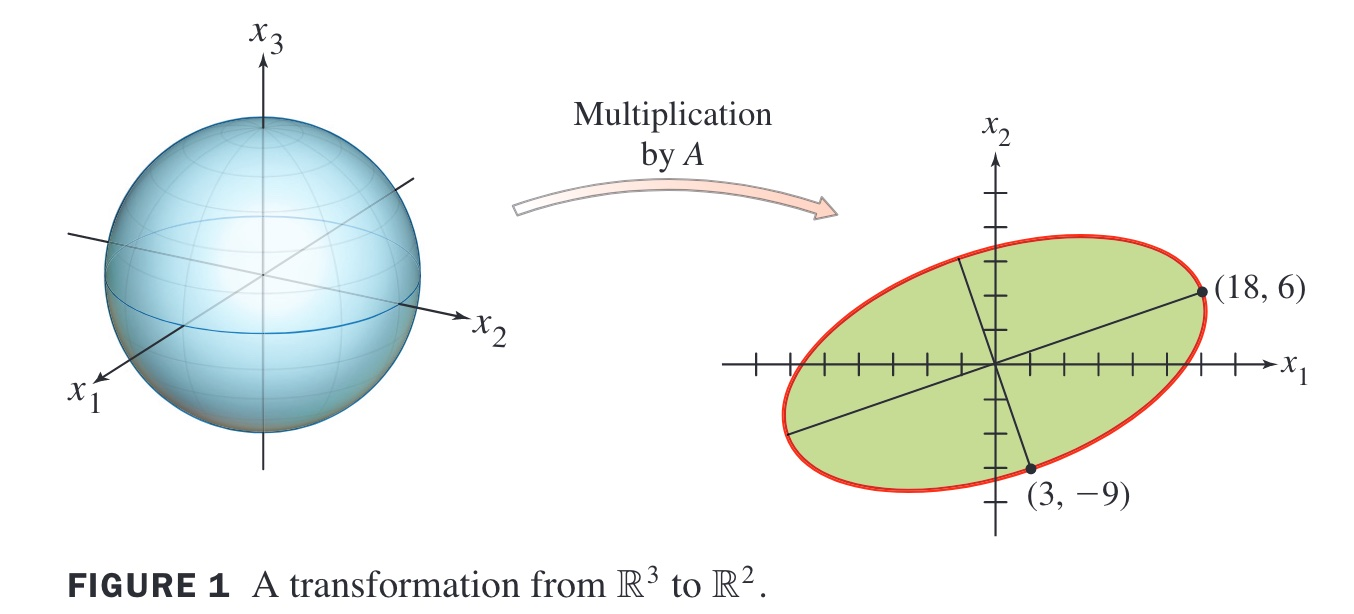
\includegraphics[width=0.8\textwidth]{svd-ex1}

    To make \(||Ax||\) maximum, also means to make \(||Ax||^2\) maximum, notice that:
    \[
        ||Ax||^2 = (Ax)^TAx = x^TA^TAx = x^T(A^TA)x
    \]
    calculating \(A^TA\) we have:
    \[
        A^TA = \begin{bmatrix}
            4 &  8 \\
            11 &  7 \\
            14 &  -2 \\
        \end{bmatrix}
        \begin{bmatrix}
            4 & 11 &  14 \\
            8 & 7 &  -2 \\
        \end{bmatrix}
        = \begin{bmatrix}
            80 & 100 &  40 \\
            100 & 170 &  140 \\
            40 & 140 &  200 \\
        \end{bmatrix}
    \]

    The eigenvalues for that are:
    \[
        \lambda_1 = 360: \begin{bmatrix}
             1/3 \\
             2/3 \\
             2/3 \\
        \end{bmatrix};
        \quad
        \lambda_2 = 90: \begin{bmatrix}
             -2/3 \\
             -1/3 \\
             2/3 \\
        \end{bmatrix};
        \quad
        \lambda_3 = 0: \begin{bmatrix}
             2/3 \\
             -2/3 \\
             1/3 \\
        \end{bmatrix}
    \]

    The maximum value is the greatest eigenvalue \(\lambda_1\) of \(A^TA\). Also, the maximum value is attained at a unit eigenvector of \(A^TA\) corresponding to \(\lambda_1\).   

    Thus the maximum \(||Ax||\) is \(\sqrt{360} = 6\sqrt{10}\) when \(x = \begin{bmatrix}
         1/3 \\
         2/3 \\
         2/3 \\
    \end{bmatrix}\)  
\end{eg}

To make the above example work, I actually omitted an important theorem (In the book, it is the Theorem 6 in Section 7.3).
    
\begin{theorem}
    Let A be a symmetric matrix, and define m and M like following:
    \[
        m = min\{x^TAx: ||x|| = 1\}, M = max\{x^TAx: ||x|| = 1\}
    \]
    Then M is the greatest eigenvalue \(\lambda_1\) of A and m is the least eigenvalue of A. 
    The value of \(x^TAx\) is M when x is a unit eigenvector \(u_1\) corresponding to M. The value of \(x^TAx\) is m when x is the unit eigenvector corresponding to m.   
\end{theorem}
\begin{proof}
    I will prove the M part here.

    After change of variable: x = Py, we know that \(x^TAx = y^TDy\). 

    Also, the norm of y, \(||y||^2 = y^Ty = y^TIy = y^TP^TPy = (Py)^TPy = ||Py||^2 = ||x||^2\), that is \(||x|| = 1\) if and only if \(||y|| = 1\).   

    Suppose the eigenvalues of A makeup a diagonal matrix:
    \[
        D = \begin{bmatrix}
            a & 0 & 0 \\
            0 & b & 0  \\
            0 & 0 & c \\
        \end{bmatrix}, a \geq b \geq c
    \]

    We have:
    \begin{align*}
        x^TAx &= y^TDy \\
            &= ay_1^2 + by_2^2 + cy_3^2 \\
            &\leq ay_1^2 + ay_2^2 + ay_3^2 \\
            &= a(y_1^2 + y_2^2 + y_3^2) \\
            &= 1
    \end{align*}
    this proves that \(M \leq a\). Can \(M = a\)? Yes, if we make \(y = e_1 = (1, 0, 0)\), then \(M = a\).  
\end{proof}


\begin{remark}
    Also, for the example, we can also use change the variable way to solve that:
    Suppose \(y = Px\), we can change \(x^T(A^TA)x\)  to \(y^TDy\) because \(A^TA\) is a symmetric matrix.  
    Notice that the diagonal matrix is \(\begin{bmatrix}
        360 & 0 &  0 \\
        0 & 90 &  0 \\
        0 & 0 &  0 \\
    \end{bmatrix}\) so the result is \(360y_1^2 + 90y_2^2\). 

    Because we still keep that \(||y|| = 1\) that is \(y1_2 + y_2^2 = 1\), to maximum the result, we can select \(y_1 = 1\) and \(y_2 = 0\) then the maximum result is 360, which makes maximum \(||Ax|| = 6\sqrt{10}\).    
\end{remark}

\subsection{The Singular Values of an m x n Matrix}

\begin{definition}
    The \textbf{singular values}  of A are the square roots of the eigenvalues of \(A^TA\), noted as \(\sigma_1, \cdots ,\sigma_n\), that is \(\sigma_i = \sqrt{\lambda_i}\) for \(1 \leq i \leq n\). 

    \begin{remark}
        The prerequisite for this is that all eigenvalues of \(A^TA\) is non-negative, and it is easy to prove:
            \begin{align*}
                ||Av_i||^2 & = (Av_i)^TAv_i \\
                    & = v_i^T A^TA v_i \\
                    & = v_i^T \lambda_i v_i \tag{\(\lambda_i\) is the eigenvalue of \(A^TA\) }\\ 
                    & = \lambda_i \tag{\(v_i\) is unit vector }
            \end{align*}
        
    \end{remark}

    \begin{remark}
        The lengths of singular values of \(A\) is the lengths of the vectors \(Av_1, \cdots, Av_n\). 
    \end{remark}
\end{definition}

\begin{theorem}\label{theorem: 7.4.9}
    Suppose \(\{ v_1, \cdots, v_n \} \) is an orthogonal basis of \(\R^n\) consisting of eigenvectors of \(A^TA\), arranged so that the corresponding eigenvalues of \(A^TA\) satisfy \(\lambda_1 \geq \cdots \geq \lambda_n\), and suppose A has \(r\)  nonzero singular values.   

    Then \(Av_1, \cdots, Av_r\) is an orthogonal basis for Col A, and rank A = r.
\end{theorem}
\begin{proof}
    (a) Proof of orthogonal (for \(i \neq j\)):

    \(Av_i \cdot Av_j = v_i^T A^TA v_j = v_i^T \lambda_j v_j = \lambda_j (v_i^T v_j) = 0\) 

    (b) They are basis for Col A

    For any \(y\) in Col A, it can be written in combination of A columns, say \(Ax\). 

    For the same reason, any \(Av_i\) is in Col A. 

    Because \(Av_i\) are orthogonal with each other, they can be used to represent any \(y\), suppose (A has n columns because \(A^TA\) is \(n \times n\)):
    \[
        y = c_1 Av_1 + c_2 Av_2 + \cdots + c_n Av_n \tag{1}
    \]  
    considering there are only r nonzero values in (1), so it can be represented as
    \[
        y = c_1 Av_1 + c_2 Av_2 + \cdots + c_r Av_r \tag{2}
    \]

    Proved \(Av_1, \cdots, Av_r\) is a basis for Col A. 

    (c) rank A = r 

    rank A = dim Col A = r
\end{proof}

\subsection{The Singular Value Decomposition}

The decomposition of A involves an \(m \times n \)  "diagonal" matrix \(\Sigma\) of the form:

\[
    \Sigma = \begin{bmatrix}
        D &  0 \\
        0 &  0 \\
    \end{bmatrix} \tag{3}
\]

where D is an \(r \times r\) diagonal matrix for some r not exceeding the smaller of m and n.

\begin{theorem}[The Singular Value Decomposition]
    Let A be an \(m \times n\) matrix with rank r. 
    Then there exists an \(m \times n\) matrix \(\Sigma\) as in (3) for which the diagonal entries in D are the first r singular values of A, \(\sigma_1 \geq \sigma_2 \geq \cdots \geq \sigma_r > 0\), 
    and there exists an \(m \times m\) orthogonal matrix \(U\) and an \(n \times n\) orthogonal matrix V such that
    \[
        A = U \Sigma V^T
    \]      
\end{theorem}
\begin{proof}
    Based on \hyperref[theorem: 7.4.9]{this theorem}, we know that \({Av_1, Av_2, \cdots, Av_r}\) is an orthogonal basis for Col A.

    Normalize each \(Av_i\)  to obtain an orthogonal basis \({u_1, u_2, \cdots, u_r}\), where 
    \[
        u_i = \dfrac{1}{||Av_i||} Av_i = \dfrac{1}{\sigma_i} Av_i
    \]
    and 
    \[
        Av_i = \sigma_i u_i \tag{4}
    \]

    Now extending \(u_1, u_2, \cdots, u_r\) to orthonormal basis \({u_1, u_2, \cdots, u_m}\) of \(\R^m\), and let
    \[
        U = \begin{bmatrix}
            u_1 & u_2 & \cdots &  u_m \\
        \end{bmatrix}
        \quad
        V = \begin{bmatrix}
            v_1 & v_2 & \cdots &  v_n \\
        \end{bmatrix}
    \]  

    By construction, U and V are orthogonal matrices, Also from (4), we have 
    \[
        AV = \begin{bmatrix}
            Av_1 & \cdots & Av_r & 0 & \cdots &  0 \\
        \end{bmatrix}
        = \begin{bmatrix}
            \sigma_1u_1 & \cdots & \sigma_ru_r & 0 & \cdots &  0 \\
        \end{bmatrix}
    \]

    And
    \[
        U\Sigma = \begin{bmatrix}
            u_1 & \cdots &  u_m \\
        \end{bmatrix}
        \begin{bmatrix}
            \sigma_1 &  & 0 & 0  \\
             & \cdots &  & 0  \\
            0 &  & \sigma_r & 0  \\
            0 & 0 & 0 &  0 \\
        \end{bmatrix}
        = \begin{bmatrix}
            \sigma_1u_1 & \cdots & \sigma_ru_r & 0 & \cdots & 0 \\
        \end{bmatrix}
    \]

    So we have \(AV = U\Sigma \implies AVV^T = U\Sigma V^T \implies A = U\Sigma V^T\) 
\end{proof}

\begin{definition}
    Any factorization \(A = U\Sigma V^T\), with U and V orthogonal, \(\Sigma \) as in (3), and positive diagonal entries in D is called a \textbf{singular value decomposition} (or \textbf{SVD}) of A. 
\end{definition}

The matrices U and V are not uniquely determined by A, but the diagonal entries of \(\Sigma\) are necessarily the singular values of A. 

The columns of U in such a decomposition are called \textbf{left singular vectors} of A, and V is called \textbf{right singular vectors} of A. 

\begin{problem}
    Show that the columns of V are eigenvectors of \(A^TA\), the columns of U are eigenvectors of \(AA^T\), and the diagonal entries of \(\Sigma\)  are the singular values of A.  
    [Hint: Use the SVD to compute \(A^TA\) and \(AA^T\).]
\end{problem}
\begin{proof}
    The assumption of the question is: U and V are orthogonal matrices, \(\Sigma\) has a diagonal matrix D like what has been shown in the beginning of the subsection. 

    Calculate \(AA^T\):
    \[
        AA^T = (U\Sigma V^T)(U\Sigma V^T)^T
            = U\Sigma V^T V \Sigma^T U^T
            = U (\Sigma \Sigma^T) U^T
    \] 
    Apparently \(\Sigma \Sigma^T\) is a diagonal matrix, and \(AA^T\) is a symmetric matrix, so the columns of U are eigenvectors of \(AA^T\), and \(\sigma_i^2 = \lambda_i\).  
\end{proof}

\subsection{Applications of the Singular Value Decomposition}

The SVD is often used to estimate the rank of a matrix.
Here are some other applications:

\begin{eg}[The Condition Number]
    Most numerical calculations involving an equation \(Ax = b\) are as reliable as possible when the SVD of A is used. 

    The two orthogonal matrices U and V do not affect the length of vectors (because \(||Ux|| = ||x||\)) or angles between vectors (because \((Ux)\cdot (Uy) = x \cdot y\)).
    Any possible instabilities in numerical calculations are identified in \(\Sigma\) (\(U \textcolor{red}{\Sigma} V x = b\)).

    If A is an *invertible* \(n \times n\) matrix, then the ratio \(\sigma_1/\sigma_n\) of the largest and smallest singular values gives the \textbf{condition number} of A.   

    \begin{remark}
        Why it needs to be invertible? Because invertible matrix won't have zero eigenvalues.    

        Proof:
        Suppose \(A\) is a matrix and has an eigenvalue 0:
        \[
            Ax = \lambda x 
            \implies 
            (A - \lambda I) x = 0 
            \implies 
            Ax = 0
            \implies
            A^{-1} A x = 0
            \implies
            x = 0
        \]
         
        But eigenvector should not be 0, thus for an invertible matrix, there should be no zero eigenvalue.
    \end{remark}
\end{eg}

\section{Applications to Image Processing and Statistics}

\subsection{Mean and Covariance}

\begin{definition}
    For two jointly distributed real-valued random variables \(X\) and \(Y\) with finite second moments, the covariance is defined as the expected value (or mean) of the product of their deviations from their individual expected values:

    \[
        cov(X, Y) = E[(X - E[X])(Y - E[Y])]
    \]
    where \(E[X]\) is the expected value of \(X\), also known as the mean of X.  
\end{definition}

In the context of discrete random variables, it can be written as:
\[
    cov(X, Y) = \dfrac{1}{n} \sum_{i = 1}^n (x_i - E(X))(y_i - E(Y)) 
\]

Let \(\begin{bmatrix}
    X_1 & \cdots & X_N  \\
\end{bmatrix}\) be a \(p times N\) matrix of observations, such as described above. The \textbf{sample mean}, M, of the observation vectors \(X_1, \cdots, X_N\) is given by
\[
    M = \dfrac{1}{N} (X_1 + \cdots + X_N)
\]

For \(k = 1, \cdots, N\), let
\[
    \hat{X}_k = X_k - M
\]

The columns of the \(p \times N\) matrix 
\[
    B = \begin{bmatrix}
       \hat{X}_1  & \hat{X}_2 & \cdots  & \hat{X}_N \\
    \end{bmatrix}    
\]
have a zero sample mean, and \(B\) is said to be in \textbf{mean-deviation form}.  

The (\textbf{sample}) \textbf{covariance matrix} is the \(p \times p\) matrix S defined by 
\[
    S = \dfrac{1}{N - 1} B B^T
\]

The \textbf{total variance}  of the data is the sum of the variance on the diagonal of S. In general, the sum of the diagonal entries of a square matrix S is called the \textbf{trace} of the matrix, written \(tr(S)\). Thus 
\[
    {total \space variance} = tr(S)
\]